\chapter{Application on a real data set}

\section{Neuroblastoma}
We consider data from \citet{oberthuer-data}, consisting of data from patients diagnosed with neuroblastoma.
Neuroblastoma is a malignant pediatric tumor that accounts for about 8\% of all childhood cancers.
One of the hallmarks of the disease is its contrasting biological behavior, which results in diverse clinical courses ranging from spontaneous regression to rapid and fatal tumor progression despite excessive treatment.

In recent years, several markers have been reported to offer valuable prognostic information.
Among these is the patient's age at diagnosis.
These markers are routinely determined by the current German neuroblastoma trial NB2004 to stratify patients into groups of high risk (50\%),
intermediate risk (10 \%) and low risk (40\%) of disease.
Therapeutic strategies vary according to these risk categories and range from a wait-and-see approach for those in the low risk group,
to intensive treatment for the high-risk group.

Clinical trials divide the individuals into risk groups with distinctive outcome.
Common clinical experience suggests that such risk classification is still suboptimal for a substantial number of patients:
The individual courses within these risk groups,
in particular those of advanced-risk patients, still vary clearly.

Originally, the data consists of two separata data sets, a larger training set, and a smaller test set, collected from Germany, and several countries, respectively.
The training set, from Germany, consists of 256 patients of the German Neuroblastoma Trials NB90-NB2004, where the patients were diagnosed between 1989 and 2004.
Patients' age at diagnosis ranged from 0 to 296 months, with a median age at 15 months.
Median follow-up for patients without fatal events was 4.5 years, with a range from 0.8 to 15.6 years.

An independent second set of 120 patients from centers in several countries were generated.
In this set, 29 of the samples were obtained from German patients enrolled in German neuroblastoma trials, while the remaining samples are from patients enrolled in national trials in other countries.
Here the age of patients at diagnosis ranged from 0 to 125 months, with a median at 15 months.
For patients without fatal events, the median follow-up time was 4.4 years, and ranged from 0.4 to 18.1 years.

In keeping with \citet{bovelstad2009}, we merge what was originally a ``training set'' of 256 patients and a ``test set'' of 120 patients into one data set.
The combining was done due to few events in the two lower NB2004 risk groups.

In total, the data consists of 362 patients suffering from neuroblastoma.
There are 9978 gene expressions measurements, which are thus from probes shared by both sets.
From each patient, we have information on their risk group according to the current German neuroblastoma trial as well as the possibly censored survival time.
This survival time was defined as time from surgery to first recurrence, and was censored at 5 years.
Median follow-up time for the patients are 3.8 years, and out of the 362 patients, 21\% died from the disease.
In addition to the risk group, the patient's age at diagnosis is recorded, resulting in two clinical covariates per patient.
9 out of the 362 observations have a missing age.
We simply remove these, and are left with a data set of 359.
In our data set, which we have received in part from Bøvelstad, we have used above or below the median age as a covariate, and not the age itself.

\citet{bovelstad2009} generated 50 random splits of training (240 patients) and test (122 patients) sets from the data.
We first generate one split of train and test data to give an example of how to interpret the estimated parameters.
Later we generate 100 random splits of training and test sets.
For each split, we carry out the boosting algorithm with the training set, and calculate the difference of deviance on the test set.

\section{Example}
The division is done by first setting a particular seed, then dividing, stratified by censoring status, into 3 almost equally sized parts.
We say that the first part is the test set, and the second and third parts are joined to make up the training set.
We then perform cross-validation on the training set.

\subsection{Cross-validation on training set}
We perform a repeated (10 times) 5-fold cross validation to find the optimal number of iterations.
We first performed a 10-fold repeated cross-validation, but this parameter search did not converge, i.e., the log-likelihood kept increasing.
Upon further inspection, we found that one of the folds was the main cause of this, as the log-likelihood for that particular fold continued to increase, even after 400 iterations, while the other folds was way into overfitting.
We concluded that splitting a training set of around 200 into 10 folds would eventually cause a problem in one of the folds, as there was too little information left.
We find $\mstop=39$ to be optimal, as seen in Figure \ref{fig:neuroblastoma-cv}.
Each dotted gray line is the sum of the negative log-likelihood of a model trained on 4 folds and applied to the last fold, as a function of iteration number.
The solid black line is the mean of these 10 gray lines, and the red vertical line indicates the optimal $\mstop$, i.e., the minimizing iteration number.
Note the impact of running the 5-fold cross-validation in a repeated fashion, as the variability in the optimal $\mstop$ is quite large.

\begin{figure}\label{fig:neuroblastoma-cv}
\caption{Repeated 5-fold cross validation on training set generated from neuroblastoma data set \citep{oberthuer-data}.}
\centering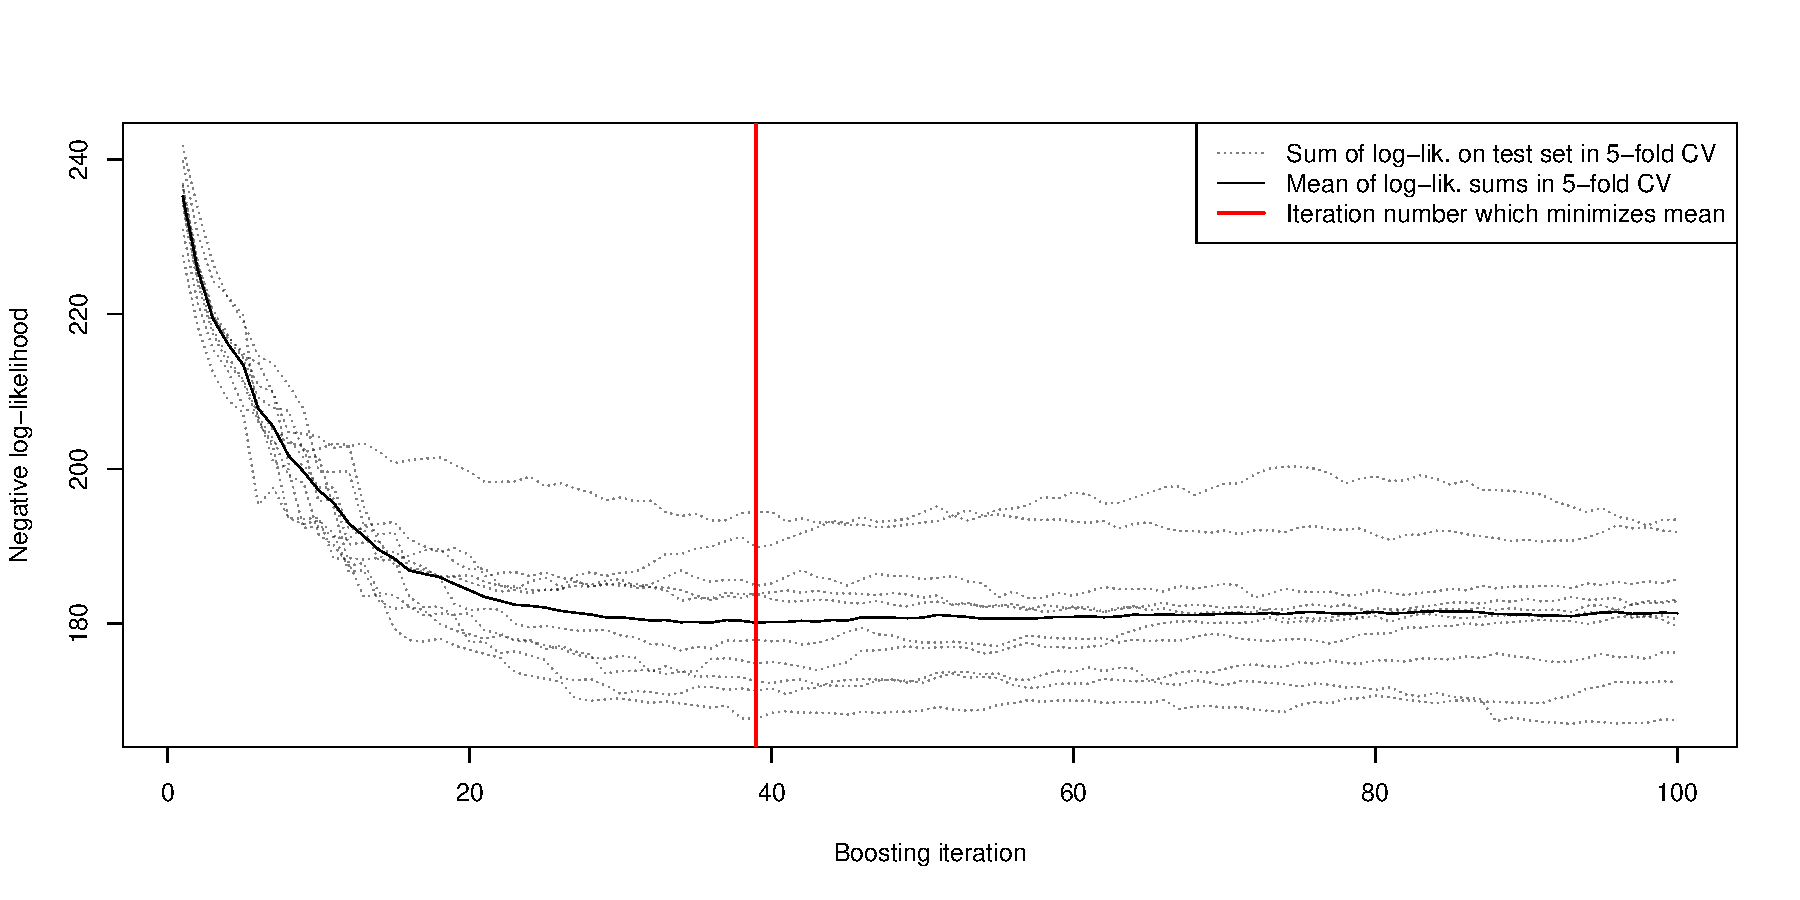
\includegraphics[scale=0.4]{figures/oberthuer_CVK5_01.pdf}
\end{figure}

\subsection{Estimation of parameters on training set, and interpretation}
After estimating the optimal stopping iteration, we run the boosting algorithm with $\mstop=39$ iterations, to estimate the model parameters on the entire training set.
The estimated parameters are reported in tables \ref{tab:oberthuer-beta} and \ref{tab:oberthuer-gamma}, for gene and clinical data, respectively.
\begin{table}\label{tab:neuroblastoma-intercepts}
\caption{Estimated intercept values}
\begin{tabular}{l|r}
Intercept parameter & Value\\
\hline
$\beta_0$ & 0.278 \\
$\gamma_0$ & 0.105
\end{tabular}
\end{table}

We first look at the intercepts, reported in table \ref{tab:neuroblastoma-intercepts}.
Here we see that the estimated intercept for the gene data, $\beta_0$, is 0.278.
We remember that in our FHT model, the vector $\bbeta$ corresponds to the initial level $y_0$ of the health process, with the log link function.
The null model, without any covariate effects, therefore has a $y_0$ of $1.32$.
Further, the intercept for the clinical data is estimated to be 0.105.
This means that the health process with the FHT interpretation that arises from our estimation is a Wiener process with a rather small initial level of 1.32, and with a \textit{positive} drift of 0.105.
Recall that the process also has a unit variance, meaning there is still a significant chance of death.
The resulting health process is
\begin{equation}
    Y(t)=1.32+W(t)\cdot0.105t,
\end{equation}
where $W(t)\sim N(0,\sqrt{t})$.
To get a feeling of the variability of this process, and potential trajectories of such a process, we plot 10 realizations of this process in Figure \ref{fig:neuroblastoma-wiener}.
Of these particular 10 processes, 7 processes at some point go below 0.
In the FHT interpretation, then, these health processes would cause a death, or, a recurrence of the neuroblastoma cancer.
In a previous section, in equation \eqref{eq:P-inf-FHT}, we stated the probability of an IG FHT lifetime not ending, if the drift is positive, like in our null model.
We calculate this for our estimated null model, obtaining
\begin{equation*}
    \Pr{(T=\infty)}=1-\Pr{(T<\infty)}=1-\exp{(-2\cdot 1.32\cdot 0.105)}=0.242,
\end{equation*}
meaning about three in four should have a recurrence during their lifetime.
For our training set, 50 out of 234 are observed events, meaning 21.4\% have died.
Note that this is with a medium follow-up of 4.5 years.
This is still a bit off from the null model prediction of the cure rate, but in any case, our model predicts a non-zero proportion of long-term survivors.
\begin{figure}\label{fig:neuroblastoma-wiener}
\caption{Wiener processes with parameters $y_0=1.32$ and $\mu=0.278$, corresponding to the estimated null model from neuroblastoma data set \citep{oberthuer-data}.}
\centering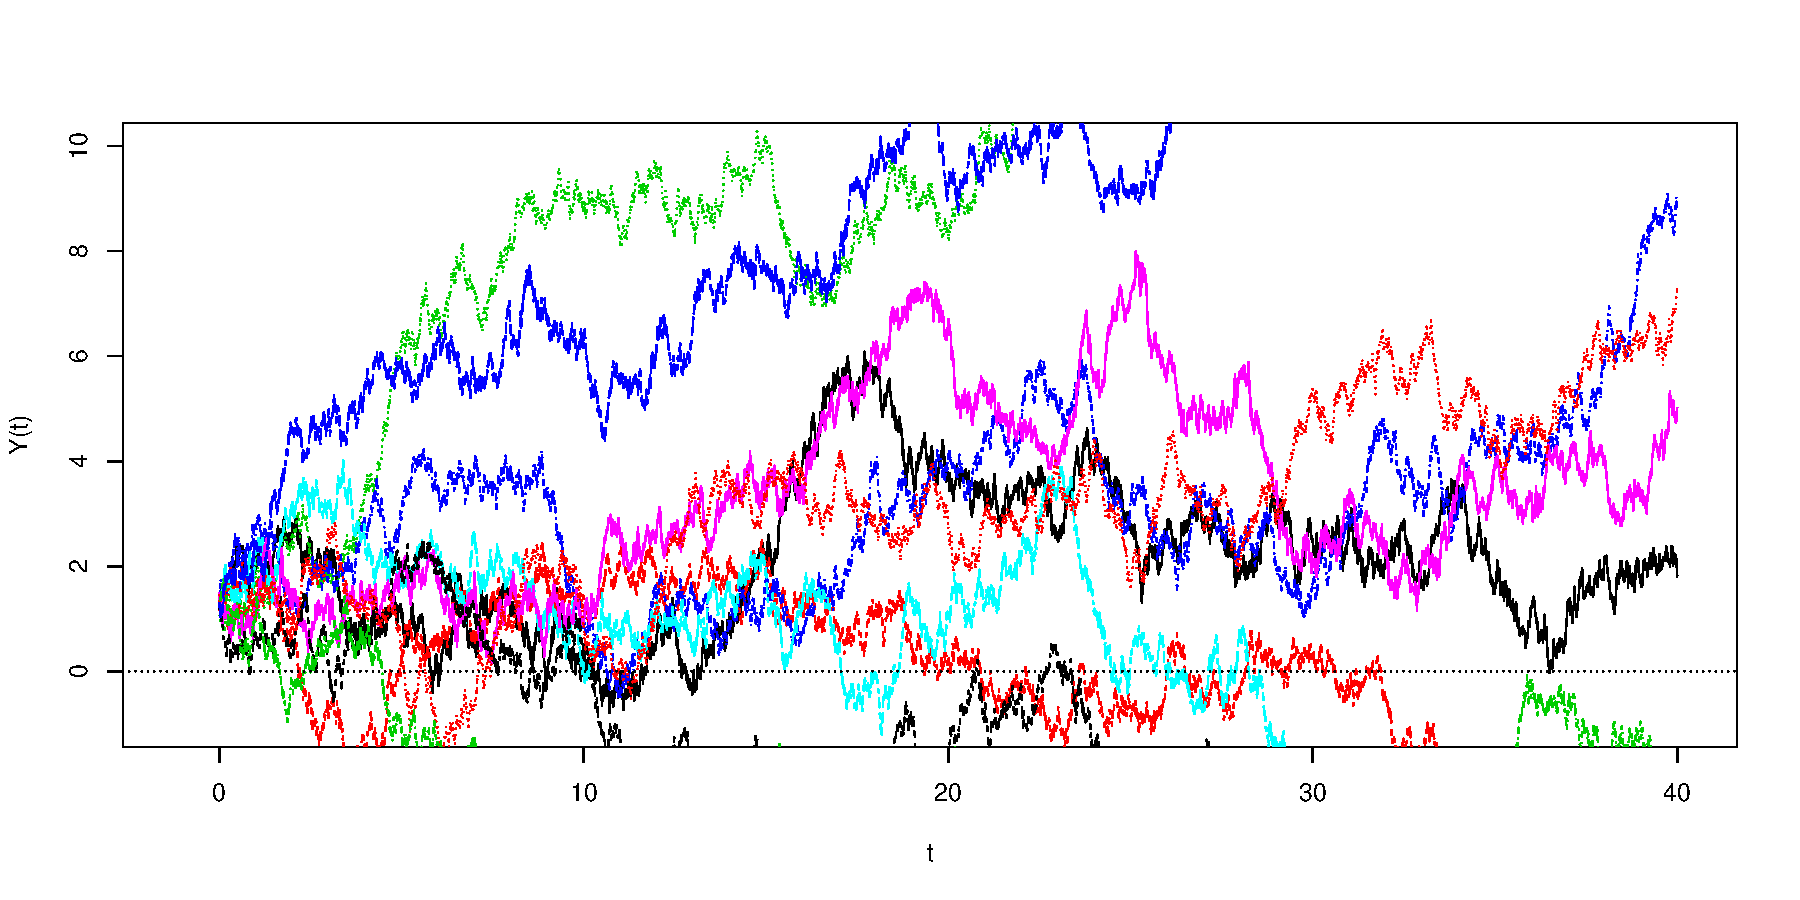
\includegraphics[scale=0.4]{figures/oberthuer-wiener-procs.pdf}
\end{figure}

Recall that what we are looking at is when, if ever, will a neuroblastoma patient have a recurrence, after a surgery.
The initial level of the Wiener process is therefore the health level of a patient at surgery.
Their health is obviously quite precarious, as neuroblastoma is a malignant cancer, and therefore it might make sense that the initial level is quite low.
However, the survival probability of patients vary, and most will, as estimated by our model, survive.
Keep also in mind that these are young children.
Therefore the health level of an average patient should in fact increase, when looking at a small time frame (as opposed to the time frame of an entire human life).

Let us further look at estimated covariate effects.
Before performing boosting, we centered and scaled each column of the covariate matrices, meaning that if you look at the covariate $j$, we have that the mean is (approximately) 0,
\begin{equation}
    \overline{x}_j=\frac{1}{n}\sum_{i=1}^n x_{i,j}\approx 0,
\end{equation}
and the standard error is approximately 1,
\begin{equation}
    s_j=\frac{1}{n}\sum_{i=1}^n (x_{i,j}-\overline{x}_j)^2\approx 1.
\end{equation}
See a previous section for an explanation of why centering and scaling is important.
For the gene expressions, this is not particularly important with regards to interpretation.
However, to properly consider the interpretation of the estimated parameters corresponding to the clinical measurements, we should
scale these back to their original scale.
For example, the covariate corresponding to risk, namely $\gamma_1$, is originally either 0 or 1, depending on the covariate.
After transforming, these are X and X, respectively.
This is therefore done in that table, table \ref{tab:oberthuer-gamma}.
We see that the model has selected both variables as informative.
The most striking result here is the large parameter corresponding to risk.
For those individuals designated as high-risk, the drift parameter is
\begin{equation}
    \mu=0.105-0.351+0.005\cdot x_{\text{age}}\approx-0.200,
\end{equation}
where $x_{\text{age}}$ is the age of the patient at diagnosis.
In particular, note that this drift will be negative for all patients.
The effect of age is positive, but the parameter is so small as to not impact the sign of the drift. \todo[inline]{CHECK!}
This means that the model predicts that all high-risk individuals will eventually have a recurrence of neuroblastoma cancer.
This seems to harmonize with the fact that these are indeed characterized as having a high risk.
Remember here that this classification of risk is done before the fact, so there is no chance of a hindsight bias.

\begin{table}
\caption{Results of estimated gene coefficients on neuroblastoma data \citep{oberthuer-data}.}
\label{tab:oberthuer-beta}
\begin{tabular}{l|r}
$j$ & $\beta_j$ \\
\hline
0    &  0.278 \\
361  & -0.006 \\
1283 &  0.007 \\
1294 & -0.005 \\
1477 & -0.006 \\
1790 & -0.007 \\
2647 & -0.014 \\
2733 &  0.009 \\
2783 & -0.013 \\
2974 & -0.010 \\
3153 &  0.010 \\
3936 &  0.029 \\
6178 & -0.009 \\
6832 &  0.005 \\
7491 &  0.028 \\
9504 &  0.008 \\
9574 & -0.005 \\
9978 & -0.006
\end{tabular}
\end{table}

\begin{table}
\caption{Results of estimated clinical coefficients on neuroblastoma data \citep{oberthuer-data}.}
\label{tab:oberthuer-gamma}
\begin{tabular}{l|rr}
$j$ & $\gamma_j$ & Properly scaled $\gamma_j$\\
\hline
0 &  0.105 &  \\
1 &  -0.351 & -0.708 \\
2 &   0.005 & 0.104
\end{tabular}
\end{table}

To get proper effect, do ...

We observe that 17 genes have been selected. Some effects are estimated to be positive, some to be negative.
Again, these gene expression measurements have been centered and scaled.
However, a larger parameter does not necessarily mean that the effect of this gene is larger than others, as that still depends on the distribution of these.
We could for example compare the model to a clinical-only model, to see the effect of genes vs clinical.

Finally, we calculate the log-likelihood on the test set, with the model estimated from the training set, and similarly using the estimated null model of the training set.
We use this to calculate the difference of deviance on the test set and obtain -9.64.

\section{Difference in deviance}
The difference in deviance between a fitted model and the null model containing no covariates is given by
\begin{equation*}
    d=-2\left(l^{\text{test}}(\bbeta_{\text{train}})-l^{\text{test}}(\0)\right),
\end{equation*}
where $l^{\text{test}}(\bbeta)$ is the likelihood attained with covariate vector $\beta$ on the test set.
The performance of a model is good when the difference in deviance is small.

In some of the results in this section, we end up with a \textit{positive} difference of deviance, which means that the null model performed better than the estimated model.
This sounds weird.
However, this will happen if the model estimated on the training set has estimated parameters which are in the \textit{opposite} direction of those in the test set.
Thus the null model will perform better than the estimated model.

\section{Comparing a clinical-only model to a full model}
We now generate 100 splits of training and test sets.
We perform the same method as above, estimating parameters based on the training set, and calculating deviance on the test set, using those parameters.
Our boosting method offers a simple way to combine clinical and genetic data in estimating.
We can use this to compare how our model performs when using only the clinical data, and when using the full data.
A method proposed in \citet{bovelstad2007}. Used in \citep{bovelstad2009}.
The median of difference of deviance as main measure of interest, and it is -35.53 for the full model, and -24.82 for the clinical model.
See Figure \ref{fig:neuroblastoma-deviances} for a boxplot of these.

\begin{figure}\label{fig:neuroblastoma-deviances}
\caption{Difference in deviance when using a clinical-only model with only boosting $\mu$ and a full model.}
\centering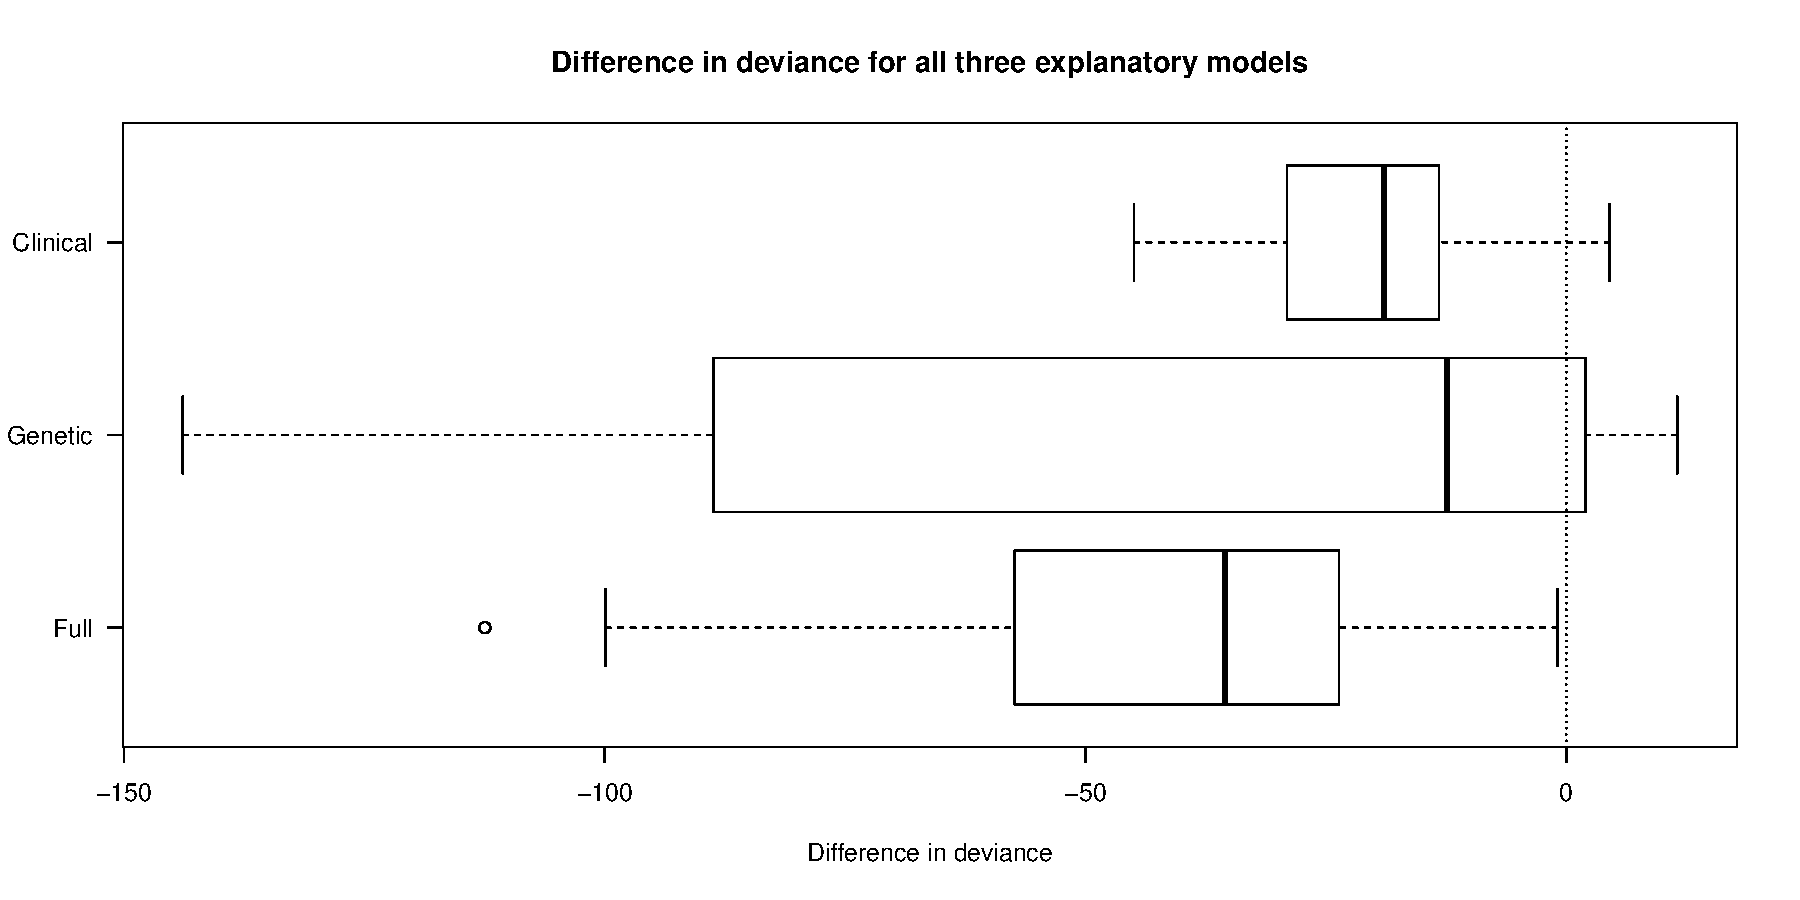
\includegraphics[scale=0.4]{figures/deviance_all_boxplot_w_title.pdf}
\end{figure}



\section{Colon cancer}
We now consider data originating from \citet{marisa-data}, consisting of patients diagnosed with colon cancer.
Colon cancer is the third most common cancer, and the fourth leading cause of cancer death worldwide \citep{marisa-data}.
Pathological staging is the only prognostic

The French national CIT program involves a multicenter cohort of 750 patients with stage I to IV CC.

About the data.

We remove observations where any covariate is missing.

We have four clinical measurements.
These are sex, which is coded as a dummy variable $x_{\text{sex}}\in\{-1,1\}$, age, subtype, and finally stage.

In the original data set, some survival times are originally 0.
We first tried setting these to $10^{-9}$, but it resulted in numerical instability when using numerical optimization to find the maximum likelihood intercepts.
We then tried setting these successively to $10^{-9},\,10^{-8},\,\cdot$, and not until 0.1 did we achieve numerical stability.
Note that this likely has a large effect on the estimated parameters.